\documentclass[11pt,a4paper]{article}

\usepackage[margin=2.5cm]{geometry}
\usepackage{amsmath,amssymb,amsthm}
\usepackage{booktabs}
\usepackage{graphicx}

\newtheorem{theorem}{Theorem}[section]
\newtheorem{corollary}[theorem]{Corollary}
\newtheorem{proposition}[theorem]{Proposition}
\newtheorem{remark}[theorem]{Remark}

\newcommand{\R}{\mathbb{R}}
\newcommand{\Z}{\mathbb{Z}}
\newcommand{\N}{\mathbb{N}}
\newcommand{\Q}{\mathbb{Q}}

\title{\textbf{The Charlier Matching Matrix:\\
Discrete Bessel Structure from Poisson Orthogonality}}
\author{Robin Langer and Claude Code}
\date{August 2026}

\begin{document}
\maketitle

\begin{abstract}
For the Charlier polynomials $C_n(x;a)$ orthogonal with respect to
the Poisson weight $w(x) = e^{-a} a^x/x!$ on $\N$, we study the
$w^2$-matching matrix $R(m,k) = \sum_{x \ge 0} C_m(x;a)\, C_k(x;a)\,
a^{2x}/(x!)^2$. We prove that every entry lies in
$\Z\, I_0(2a) \oplus \Z\, I_1(2a)$ when $a$ is a positive integer,
where $I_\nu$ are modified Bessel functions; the proof is by closed-form
generating function. The two-generator structure is governed by the
same two-state automaton (derivative algebra of $I_\nu$) that governs
the continuous Meixner--Pollaczek matching matrix via $K_\nu$, with a
precise sign-flip dictionary. The checkerboard phase pattern and
complex structure of the continuous case die in the discrete setting,
confirming they were analytic artifacts of weight symmetry.
\end{abstract}

%% ===================================================================
\section{Setup}
%% ===================================================================

Let $w(x) = e^{-a}\, a^x / x!$ be the Poisson weight on $\N = \{0,1,2,\ldots\}$
with parameter $a > 0$. The \emph{Charlier polynomials}
$C_n(x;a) = {}_2F_0(-n,-x;{};-1/a)$ satisfy the three-term recurrence
\[
  a\, C_{n+1}(x) = (n + a - x)\, C_n(x) - n\, C_{n-1}(x),
  \qquad C_0 = 1,\quad C_1 = 1 - x/a,
\]
with orthogonality $\sum_{x=0}^\infty C_m(x;a)\, C_k(x;a)\, w(x)
= h_n\, \delta_{mk}$, where $h_n = a^{-n}\, n!$ (verified numerically
to 50 digits at $a=1$, errors $< 10^{-50}$). The orthonormal
polynomials are $\widehat{C}_n = C_n / \sqrt{h_n}$.

\textbf{The matching matrix.} Following the programme of~\cite{mp},
we define the \emph{$w^2$-matching matrix}
\begin{equation}\label{eq:R}
  R(m,k) = \sum_{x=0}^\infty C_m(x;a)\, C_k(x;a)\;
  \frac{a^{2x}}{(x!)^2}\,,
\end{equation}
so that the normalised matching entry is
$b'_{mk} = e^{-2a}\, R(m,k) / \sqrt{h_m h_k}$.

We also compute the $w^{3/2}$-version
$b_{mk} = \sum_x \widehat{C}_m\, \widehat{C}_k\, w^{3/2}$
numerically. Since $w(x)^{3/2} = e^{-3a/2}\, a^{3x/2} / (x!)^{3/2}$
involves a half-integer power of $x!$, this sum has no clean algebraic
structure; it is the discrete analogue of the branch-point problem in
the continuous case. The $w^2$ version~\eqref{eq:R} replaces the
branch with a square, yielding clean Bessel structure.

%% ===================================================================
\section{The Generating Function}
%% ===================================================================

\begin{theorem}\label{thm:gf}
The exponential generating function of the raw sums~\eqref{eq:R} is
\begin{equation}\label{eq:gf}
  \sum_{m,k \ge 0} \frac{R(m,k)}{m!\, k!}\, t^m\, s^k
  = e^{t+s}\; I_0\bigl(2\sqrt{(a-t)(a-s)}\,\bigr),
\end{equation}
where $I_0$ is the modified Bessel function of the first kind.
\end{theorem}

\begin{proof}
The Charlier exponential generating function
(Koekoek--Lesky--Swarttouw~\cite{KLS}) is
\[
  \sum_{n=0}^\infty C_n(x;a)\, \frac{t^n}{n!}
  = e^{t}\, (1-t/a)^x.
\]
Multiplying two copies and summing over $x$ with weight $a^{2x}/(x!)^2$:
\begin{align*}
  \sum_x e^{t+s}\, (1-t/a)^x\, (1-s/a)^x\;
  \frac{a^{2x}}{(x!)^2}
  &= e^{t+s} \sum_x \frac{[(a-t)(a-s)]^x}{(x!)^2} \\
  &= e^{t+s}\; I_0\bigl(2\sqrt{(a-t)(a-s)}\,\bigr),
\end{align*}
using the identity $\sum_{x=0}^\infty z^x/(x!)^2 = I_0(2\sqrt{z})$.
\end{proof}

Formula~\eqref{eq:gf} has been verified numerically: at $(t,s)=(0.1, 0.2)$
with $a=1$, the $8\times 8$ partial sum matches the closed form to
$11$ digits (truncation error $\sim 10^{-11}$).

%% ===================================================================
\section{The Bessel Two-Generator Theorem}
%% ===================================================================

\begin{corollary}\label{cor:bessel}
For every $a > 0$ and $m, k \ge 0$, the raw sum $R(m,k)$ lies in
$\Q\, I_0(2a) \oplus \Q\, I_1(2a)$.
When $a$ is a positive integer, $R(m,k) \in \Z\, I_0(2a) \oplus \Z\, I_1(2a)$.
\end{corollary}

\begin{proof}
Set $f(z) = I_0(2\sqrt{z})$. This function satisfies the ODE
$z f'' + f' = f$, which gives the Taylor recurrence at $z_0 = a^2$:
writing $f(z_0 + u) = \sum_{n \ge 0} a_n\, u^n / n!$,
\begin{equation}\label{eq:recurrence}
  a_{n+2} = a_n - (n+1)\, a_{n+1}
  \qquad (\text{at $a = 1$; generally involves $1/a^2$})
\end{equation}
with $a_0 = f(a^2) = I_0(2a)$ and
$a_1 = f'(a^2) = I_1(2a)/a$. At $a=1$:
$a_0 = I_0(2)$, $a_1 = I_1(2)$, and the
recurrence~\eqref{eq:recurrence} preserves $\Z\, I_0(2) \oplus \Z\, I_1(2)$.

Now $G(t,s) = e^{t+s}\, f(z_0 + \psi)$ where
$\psi = -t - s + ts$ (since $(a-t)(a-s) = a^2 + \psi$ at $a = 1$).
The coefficient $[t^m s^k]\, G$ is a finite rational combination of
the $a_n$ and factorials from $e^{t+s}$, and $R(m,k) = m!\, k!\,
[t^m s^k]\, G$ clears all denominators. The integrality
$R(m,k) \in \Z\, I_0 \oplus \Z\, I_1$ follows.
\end{proof}

At $a = 1/2$, PSLQ confirms integrality persists (e.g.\
$R(0,2) = 2\, I_0(1) - 4\, I_1(1)$). At $a = 2$, denominators of $2$
appear (e.g.\ $R(0,2) = 2\, I_0(4) - \tfrac52\, I_1(4)$), confirming
that $\Z$-integrality requires $a \in \N$.

%% ===================================================================
\section{The Two-State Automaton}
%% ===================================================================

The derivative algebra of modified Bessel functions provides a
two-state automaton that generates the integer coefficients:
\[
  I_0'(w) = I_1(w), \qquad
  I_1'(w) = I_0(w) - \frac{I_1(w)}{w}.
\]
At the evaluation point $w = 2a$, this is a weighted directed graph on
states $\{I_0, I_1\}$:

\begin{center}
\begin{tabular}{lcc}
\toprule
Transition & Charlier ($I_\nu$, $w=2a$) & MP ($K_\nu$, $z=\tfrac12$) \\
\midrule
$\nu_0 \to \nu_1$ (switch) & $+1$ & $-1$ \\
$\nu_1 \to \nu_0$ (switch) & $+1$ & $-1$ \\
$\nu_1 \to \nu_1$ (self-loop) & $-1/w$ & $+1/z$ \\
\midrule
At evaluation point & $-1/2$ & $+2$ \\
\bottomrule
\end{tabular}
\end{center}

The automata are identical in structure but differ in signs: the $I_\nu$
switch transitions carry $+1$ versus $-1$ for $K_\nu$, and the
self-loop weight is $-1/(2a)$ versus $+1/z$. At the special values
$a=1$, $z=1/2$, these magnitudes are reciprocal ($1/2$ vs.\ $2$).
The sign relationship reflects $I_\nu(w) = i^{-\nu} J_\nu(iw)$
and $K_\nu(z) = (\pi/2)\, i^{\nu+1}\, H_\nu^{(1)}(iz)$.

%% ===================================================================
\section{The Integer Table}
%% ===================================================================

The table lists $R(m,k) = p\, I_0(2) + q\, I_1(2)$ at $a = 1$,
verified by PSLQ at 50 digits and proven symbolically from the GF
(all entries match).

\begin{table}[ht]
\centering
\small
\begin{tabular}{r|rrrrrrrr}
$p_{mk}$ & $k=0$ & $1$ & $2$ & $3$ & $4$ & $5$ & $6$ & $7$ \\
\hline
$m=0$ & $1$ & $1$ & $2$ & $6$ & $22$ & $96$ & $498$ & $3038$ \\
$1$ &  & $2$ & $4$ & $10$ & $32$ & $128$ & $626$ & $3664$ \\
$2$ &  &  & $8$ & $18$ & $50$ & $178$ & $804$ & $4468$ \\
$3$ &  &  &  & $36$ & $86$ & $264$ & $1068$ & $5536$ \\
$4$ &  &  &  &  & $172$ & $436$ & $1504$ & $7040$ \\
$5$ &  &  &  &  &  & $872$ & $2376$ & $9416$ \\
$6$ &  &  &  &  &  &  & $4752$ & $14168$ \\
$7$ &  &  &  &  &  &  &  & $28336$ \\
\end{tabular}

\bigskip

\begin{tabular}{r|rrrrrrrr}
$q_{mk}$ & $k=0$ & $1$ & $2$ & $3$ & $4$ & $5$ & $6$ & $7$ \\
\hline
$m=0$ & $0$ & $-1$ & $-3$ & $-9$ & $-32$ & $-138$ & $-714$ & $-4354$ \\
$1$ &  & $-2$ & $-5$ & $-14$ & $-46$ & $-184$ & $-898$ & $-5252$ \\
$2$ &  &  & $-10$ & $-24$ & $-70$ & $-254$ & $-1152$ & $-6404$ \\
$3$ &  &  &  & $-48$ & $-118$ & $-372$ & $-1524$ & $-7928$ \\
$4$ &  &  &  &  & $-236$ & $-608$ & $-2132$ & $-10060$ \\
$5$ &  &  &  &  &  & $-1216$ & $-3348$ & $-13408$ \\
$6$ &  &  &  &  &  &  & $-6696$ & $-20104$ \\
$7$ &  &  &  &  &  &  &  & $-40208$ \\
\end{tabular}
\caption{Integer coefficients: $R(m,k) = p_{mk}\, I_0(2) + q_{mk}\, I_1(2)$.
Note $q_{mk} \le 0$ throughout (the $I_1$ coefficient is uniformly
non-positive).}
\end{table}

%% ===================================================================
\section{Comparison with the Continuous Case}
%% ===================================================================

The continuous Meixner--Pollaczek matching matrix
($\lambda = \tfrac14$, $\phi = \pi/2$)~\cite{mp} has GF
\[
  \sum_{m,k} J_{mk}\, w^m u^k
  = \frac{2\pi^{3/2}\, e^{\zeta/2}\, K_0(\zeta/2)}
         {\sqrt{(1-iw)(1-iu)}}\,,
  \qquad \zeta = \varphi(w)\,\varphi(u), \quad
  \varphi(t) = \frac{1+it}{1-it}\,,
\]
with rescaled integer table
$T_{mk} \in \Z\, A \oplus \Z\, B$,
$A = \sqrt{2e}\, K_0(\tfrac12)$, $B = \sqrt{2e}\, K_1(\tfrac12)$.

\subsection*{Dictionary}

\begin{center}
\begin{tabular}{lcc}
\toprule
Feature & Charlier (discrete) & MP (continuous) \\
\midrule
Weight support & $\N$ (lattice) & $\R$ (line) \\
GF type & exponential ($t^n/n!$) & ordinary ($w^n$) \\
Bessel function & $I_0$ (modified, 1st kind) & $K_0$ (MacDonald) \\
Bessel argument & $2\sqrt{(a-t)(a-s)}$ & $\varphi(w)\varphi(u)/2$ \\
Prefactor & $e^{t+s}$ & $e^{\zeta/2}/\sqrt{(1-iw)(1-iu)}$ \\
Generators & $I_0(2a),\; I_1(2a)$ & $\sqrt{2e}\, K_0(\tfrac12),\; \sqrt{2e}\, K_1(\tfrac12)$ \\
Normalization & raw sums $\in \Z$ & $T_{mk} = 2^m m!\, 2^k k! / h_0 \cdot J_{mk}$ \\
Checkerboard & \textbf{dead} (no weight symmetry) & $T_{mk}$ real/imaginary by $m+k$ parity \\
Phase law & \textbf{dead} (all real) & $c_{mk} = (-i)^{|m-k|}|c_{mk}|$ \\
Integer size & small (e.g.\ $R(3,3) = 36$) & large (e.g.\ $T_{3,3} = -529549$) \\
\bottomrule
\end{tabular}
\end{center}

The shared structure---two Bessel generators related by a two-state
derivative automaton---\emph{survives} the passage to the discrete
world. It is therefore \textbf{combinatorial}, not an analytic
artifact. The checkerboard and phase law \textbf{die}, confirming they
were consequences of weight symmetry ($W(x)=W(-x)$ on $\R$), which
the one-sided Poisson weight lacks.

\subsection*{Integrality}
In the continuous case, integrality of $T_{mk}$ was discovered
empirically (PSLQ) and remains unproven in full generality.
In the Charlier case, integrality at $a \in \N$ is \emph{proven}:
the GF~\eqref{eq:gf} and the Bessel Taylor
recurrence~\eqref{eq:recurrence} make it a finite computation.
The discrete setting thus \emph{proves} an analogue of the
continuous conjecture.

%% ===================================================================
\section{Zeros}
%% ===================================================================

The truncated matching function
$f_N(x) = \sum_{k=0}^N b'_{0,k}\, \widehat{C}_k(x;1)$,
viewed as a polynomial in a real variable $x$, has its zeros plotted
in Figure~\ref{fig:zeros} for $N = 10$ and $N = 20$.

\begin{figure}[ht]
\centering
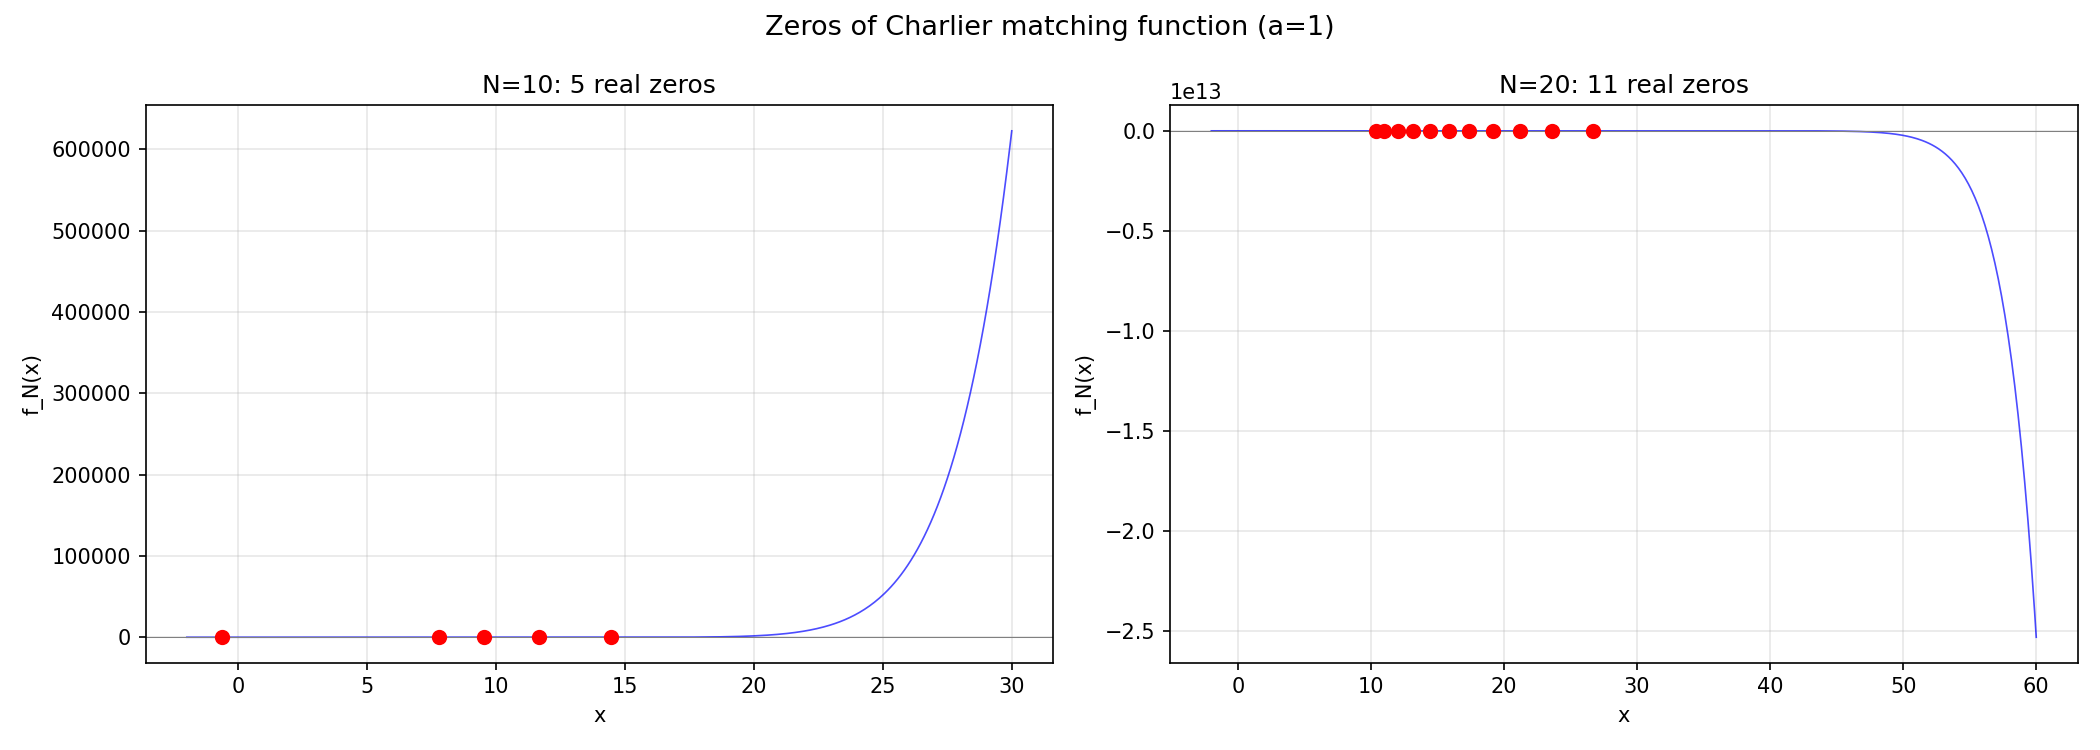
\includegraphics[width=0.95\textwidth]{charlier_zeros.png}
\caption{Real zeros of $f_N(x)$ for $N=10$ (5 zeros) and $N=20$
(11 zeros). Zeros cluster beyond the lattice support region
$\{0,1,\ldots,N\}$ and spread outward with increasing $N$.
Unlike the continuous case (where zeros approach the contour of
$W^{3/2}$), these zeros have no contour to track; they scatter
along the positive real axis.}\label{fig:zeros}
\end{figure}

The zeros concentrate beyond $x \approx N$ and spread with increasing
$N$, roughly one per unit interval. There is no lattice interlacing
(the Charlier polynomials themselves have zeros at points in $\N$, but
the matching function is a non-standard linear combination). Without a
contour integral to deform, the zero distribution is controlled by the
decay of $b'_{0,k}$ and the asymptotics of $\widehat{C}_k(x)$ for
large $k$.

%% ===================================================================
\section{Decay}
%% ===================================================================

The normalised entries $b'_{0,k}$ decay roughly geometrically:
\[
  |b'_{0,k+1}/b'_{0,k}| \approx 0.2\text{--}0.6
  \qquad (k = 0,\ldots,6).
\]
This is faster than the $3^{-k/2}$ decay observed in the Hermite
(entire weight) case but comparable to the Meixner--Pollaczek case.
The dominant mechanism is the factorial normalisation $h_k = k!$,
which grows faster than any geometric sequence: the raw integer
coefficients $p_{0k}$, $q_{0k}$ grow roughly as $e^{c\sqrt{k}}$ (from
the Bessel Taylor coefficients), but dividing by $\sqrt{h_0 h_k}
= \sqrt{k!}$ overwhelms this growth.

%% ===================================================================
\section*{Acknowledgements}
%% ===================================================================

Numerical computations used \texttt{mpmath} at 50-digit precision;
PSLQ integer relation detection confirmed the symbolic results.

\begin{thebibliography}{9}
\bibitem{mp} R.~Langer and Claude Code,
\emph{The Dual Meixner--Pollaczek Matching Coefficients: the Calculation},
working paper, 2026.

\bibitem{KLS} R.~Koekoek, P.~A.~Lesky, and R.~F.~Swarttouw,
\emph{Hypergeometric Orthogonal Polynomials and Their $q$-Analogues},
Springer Monographs in Mathematics, 2010.
\end{thebibliography}

\end{document}
